%%%%%%%%%%%%%%%%%%%%%%%%%%%%%%%%%%%%%%%%%%%%%%%%%%%%%%%%%%%%%%%%%
%                                                               %
%                       Legal Notice                            %
%                                                               %
% This document is copyright (C) Jason Gobat & Darren Atkinson	%
%                                                               %
%%%%%%%%%%%%%%%%%%%%%%%%%%%%%%%%%%%%%%%%%%%%%%%%%%%%%%%%%%%%%%%%%

\newpage{\pagestyle{empty}\cleardoublepage}

\chapter{Post-processing with {\em velvet}}
\label{velvet.solve}

\section{Solving a problem with {\em velvet}}

Depending on what you want your solution to include, there are a couple
of different ways to go about solving a \felt{} problem from within
{\em velvet}.  In addition to the standard tabular type \felt{} output (see 
section~\ref{felt_prog.output}) you can also have {\em velvet} generate
two-dimensional color shaded stress or displacement plots and/or plots 
of the structure with magnified displacements applied.  For transient 
analysis problems graphical time-displacement or time-temperature plots replace 
the ASCII versions that {\em felt} produces.  Transient structural analysis can 
also include an animation of the simulation.  For spectral analysis, graphical 
plots of the transfer functions or ouput spectra replace {\em felt}'s ASCII 
versions.  {\em velvet} can also draw graphical representations of mode shapes 
for modal analysis problems.

One way to solve a problem is to select the {\bf solve} option from the
{\bf solutions} menu.  By default, this simply generates the standard \felt{} 
output. This window will contain either the mathematical solution of
your problem or the syntax errors encountered in solving the problem.

For more control over what gets generated whenever you solve a problem
you can use the output control dialog box (Figure~\ref{velvet.output}, 
available by selecting {\bf results/output} from the {\bf solutions} menu.  
The toggle buttons in this dialog box control all of the available
solution and output options, both text and graphical.   

The three toggles at the top--left of the dialog mimick three of the
switches available in {\em felt}; they control the computations that are 
performed for modal or spectral analysis.  The {\bf felt output} toggle 
controls whether or not you want to see any of the standard textual output
that {\em felt} would generate.   If the {\bf felt output} toggle is on then 
the other three textual output toggles mimick command-line 
switches that are available in {\em felt} (see chapter~\ref{felt_prog}) to
control the printing of additional information within the textual output.  

\begin{figure}
\begin{center}
 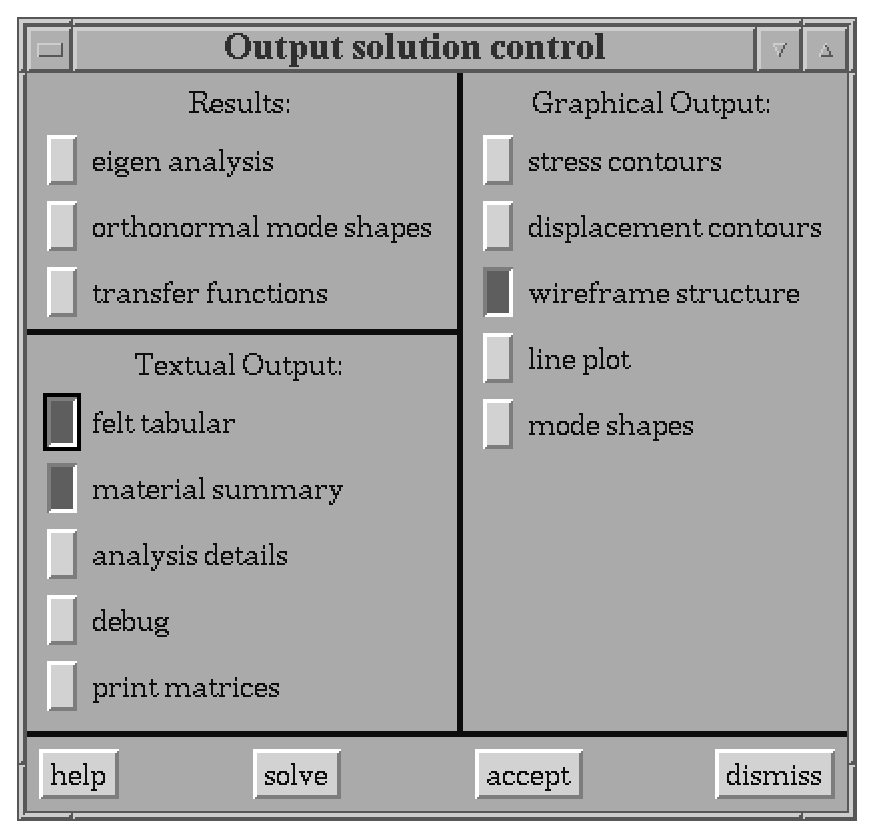
\includegraphics[width=2.59in]{figures/velvet_output}
\end{center}
\caption{The output control dialog box.}
\label{velvet.output}
\end{figure}

For graphical output, the toggles for
stress, structure and displacement plots simply allow you to automatically
invoke these post-processing options (see below) on solution.  The other two
options (time-displacement plots and mode shape plots) are only available
during a problem solution (i.e., only by selecting the appropriate toggle
in this dialog and then solving the problem).  The
{\bf line plot} option generates a graphical line plot (as opposed
to the ASCII plot that you would get with {\em felt} output) for transient
or spectral results.  A graphical time-displacement plot is 
shown in Figure~\ref{velvet.graph}.  Figure~\ref{velvet.modal} is an example of
a mode shape plot.  Note that {\em velvet} only draws a single mode 
at a time and that the regular problem geometry is drawn as an underlying 
dotted line; you can cycle forward and backward through the individual modes
using the $<$ and $>$ buttons.

\begin{figure}
\begin{center}
 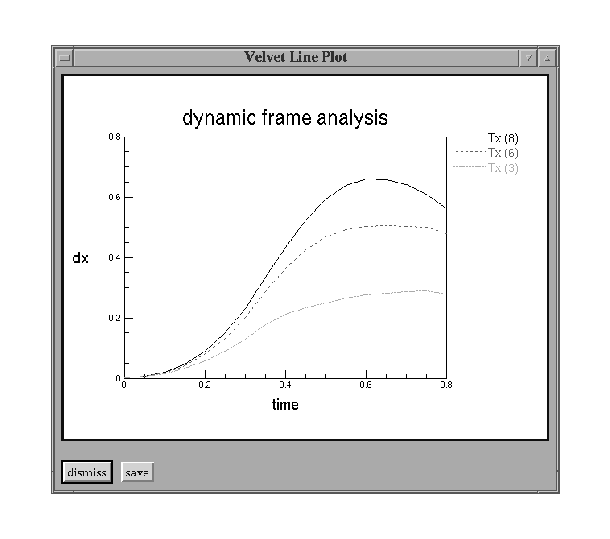
\includegraphics[width=3.73in]{figures/velvet_graph}
\end{center}
\caption{A time-displacement plot in {\em velvet}}.
\label{velvet.graph}
\end{figure}

\begin{figure}
\begin{center}
 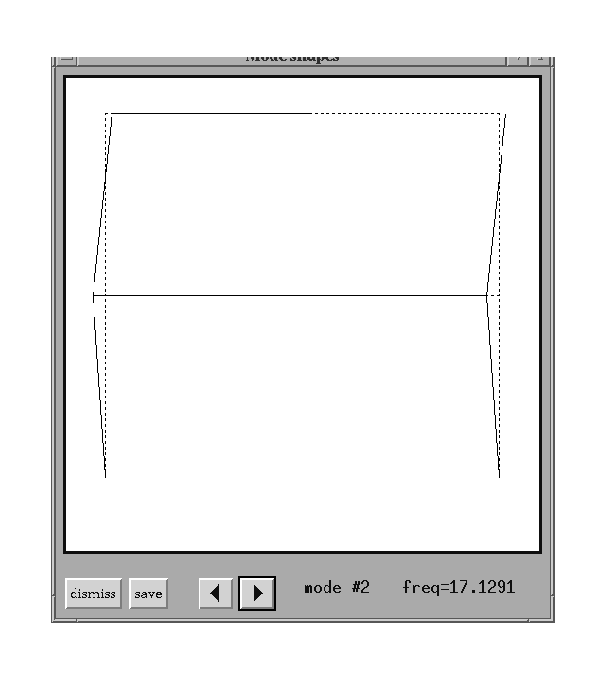
\includegraphics[width=3.14in]{figures/velvet_modal}
\end{center}
\caption{The mode shape plotting window}.
\label{velvet.modal}
\end{figure}

Given the settings in our example control box, the output for a
static model of a bicycle would be the two windows shown in 
Figures~\ref{velvet.ascii} and \ref{velvet.structure}. (The input file
for this problem can be found as {\tt bicycle\_boys.flt} in the tests
directory of the standard \felt{} distributions.)

\begin{figure}
\begin{center}
 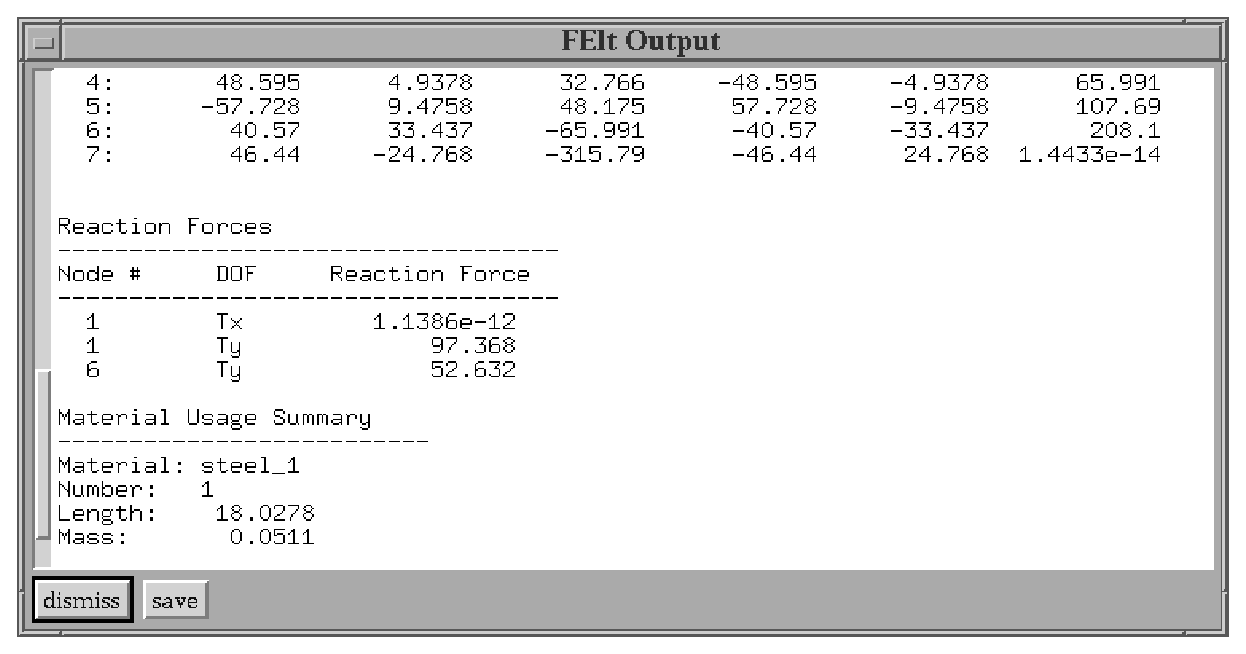
\includegraphics[width=4.0in]{figures/velvet_ascii}
\end{center}
\caption{An example of textual output from {\em velvet}.}
\label{velvet.ascii}
\end{figure}

\begin{figure}
\begin{center}
 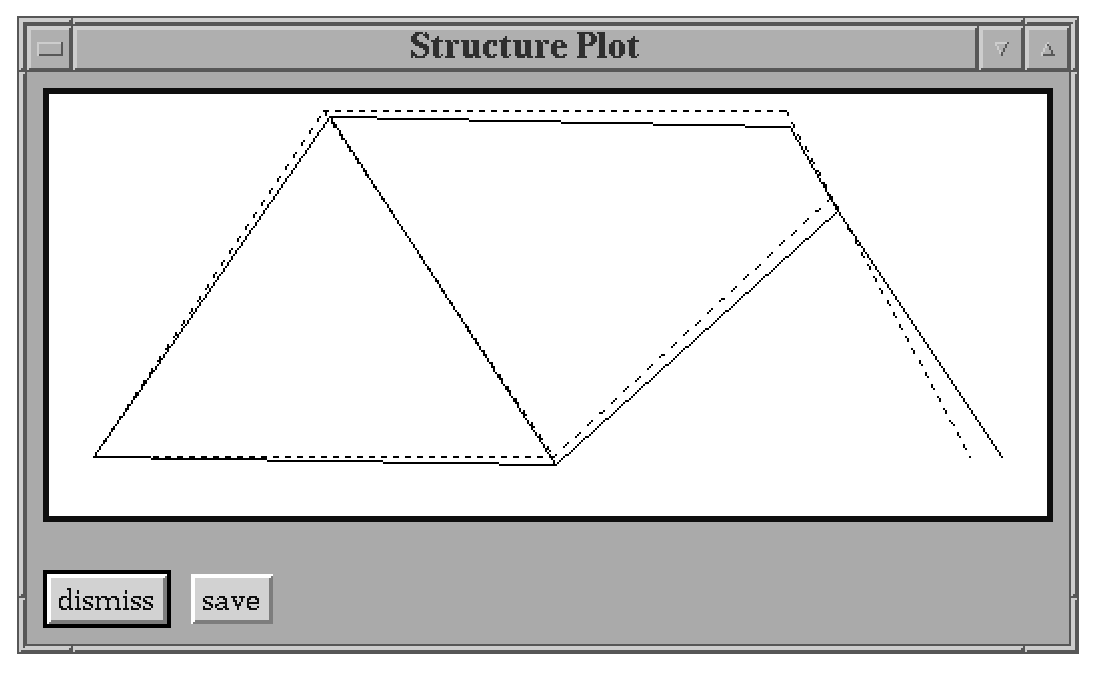
\includegraphics[width=3.13in]{figures/velvet_structure}
\end{center}
\caption{An example of a displaced structure plot.}
\label{velvet.structure}
\end{figure}

You can save any of the {\em velvet} output by clicking {\bf save} at the 
bottom of the output window.  A file dialog will 
pop-up and allow you to name the file which you wish to save to.  
Depending on the type of output, you may have the option of saving in
one of several different file formats.  Time-displacement, wireframe
structure, and mode shape plots can be saved in either XWD or PostScript 
format.  Text output can be saved as an ASCII file.  Color contours of stress 
and displacement can be saved in PPM or encapsulated PostScript (EPS) format.  

You can leave all output windows up as long as you like.  If you want to 
unview one at some point in your work, simply click {\bf dismiss}.  

For a transient analysis problem you can build a special case simulation
for animation simply by selecting {\bf animate} from the {\bf solutions}
menu.  The solution that is constructred is special in that the displacement
of all nodes in the x and y (and possibly z) translational DOF will be 
automatically recorded
for each time step.  (This is in contrast to the normal mode of solution for
a transient analysis problem in which only specially requested nodes and
DOF are recorded for output at the end of the simulation.)  Once this
complete table is built the animate window (Figure~\ref{velvet.animate}) 
will pop-up 
and you can use the playback controls to determine the speed and direction 
of the animation.  The buttons that look like rewind and fast forward
($<<$ and $>>$) are really the speed controls.  Holding them down will
slow down or speed up the animation.  The play backward and play
forward buttons ($<$ and $>$) control which direction time moves during
the animation.  You can use the stop button to freeze the structure at a given
point during the animation.  The text indicator in the right bottom corner
of the window keeps track of the elapsed time.  The animation will
repeat itself until it is either stopped or the animation window is dismissed.

\begin{figure}
\begin{center}
 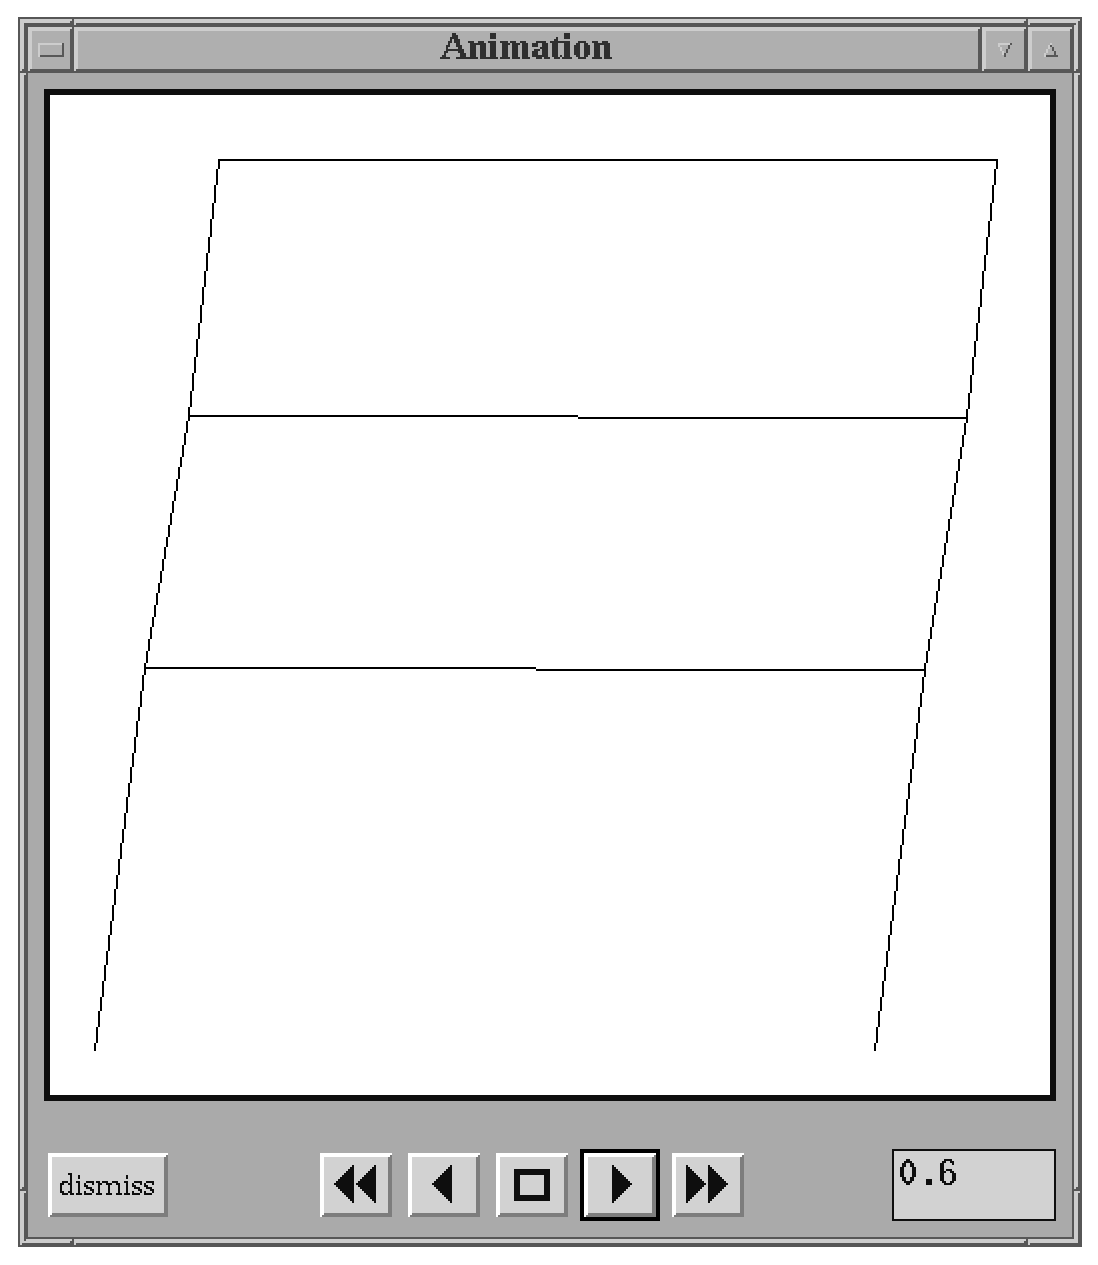
\includegraphics[width=3.10in]{figures/velvet_animate}
\end{center}
\caption{An animation in {\em velvet}}.
\label{velvet.animate}
\end{figure}

\section{Problem description and analysis parameters}

The {\tt problem description} and {\tt analysis parameters} section of
a regular \felt{} input file are mimicked in {\em velvet} by the
problem and analysis dialog box (Figure~\ref{velvet.analysis}).  This
dialog is available by selecting {\bf problem/analysis} from the 
{\bf solutions} menu.  The problem title text entry defines the header
that will be used for textual output and on graphical line
plots.  The analysis mode is defined by engaging one of the 
toggle buttons just below the problem title at the top of 
the dialog.  The mass-mode toggles below the analysis toggles allow you to 
select either consistent or lumped mass formulations for element mass 
matrices. 

For a transient structural and thermal analysis problems, there are several 
parameters which control the numerical integration in time. 
The text entries down the left side of the dialog allow you to fill in values
for these parameters in the $\gamma$, $\beta$, and $\alpha$ text
entries.  For both transient and spectral analysis the range of
time or frequency over which to perform the computations is defined by
the $start$, $stop$, and $step$ text entries.  Note that the value
for $start$ is ignored in transient analysis types.  Values for the
global Rayleigh damping proportionality constants are defined with the
$Rk$ and $Rm$ text entries.  Remember that if either of these values is
non-zero then the Rayleigh damping for this problem will be based on these
values and the global stiffness and mass matrices as opposed to elemental
material values of $Rk$ and $Rm$ and the element stiffness and mass matrices.

The DOF toggles and the node entries allow you
to define the list of nodes and which DOF at each of those nodes that you
would like to have included in the output when the problem is solved.
Click on the left and right arrow keys to scroll through the complete list
of nodes if you are interested in more than six of them.

The push buttons on the bottom of the dialog box are standard of course.
The {\bf solve} and {\bf animate} buttons are simply there as a convenience; 
pushing either button will cause the current state of the dialog to be 
registered (as if you had pushed {\bf accept}) and then the appropriate 
action to be taken just as if you had selected {\bf solve} or {\bf animate} 
from the main {\bf solutions} menu.

\begin{figure}
\begin{center}
 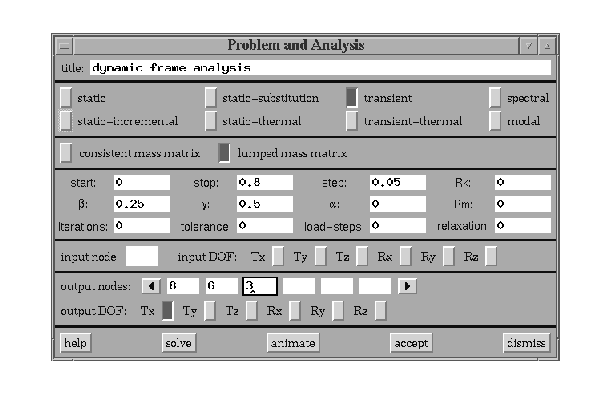
\includegraphics[width=3.15in]{figures/velvet_analysis}
\end{center}
\caption{The analysis parameters dialog box}.
\label{velvet.analysis}
\end{figure}

\section{Controlling the post-processing}

\subsection{Controlling contour plots}

The controls for color contour plots are available by selecting 
{\bf contouring} from the {\bf postprocessing} menu.  On the dialog
(Figure~\ref{velvet.contour}), there are identical controls for stress
and displacement plots.  On the stress side, the component specifies which
stress component will be plotted.  This number is element specific and must
be a valid index in the stress vector for each element type in the problem.
Consult Table~\ref{felt_prog.stress_table} for details on what the 
stress vector consists of for each element type.  For displacement plots,
the component is simply the displacement DOF that you want to see plotted.
In general, this should be one of the active global DOF for the current
problem.

\begin{figure}
\begin{center}
 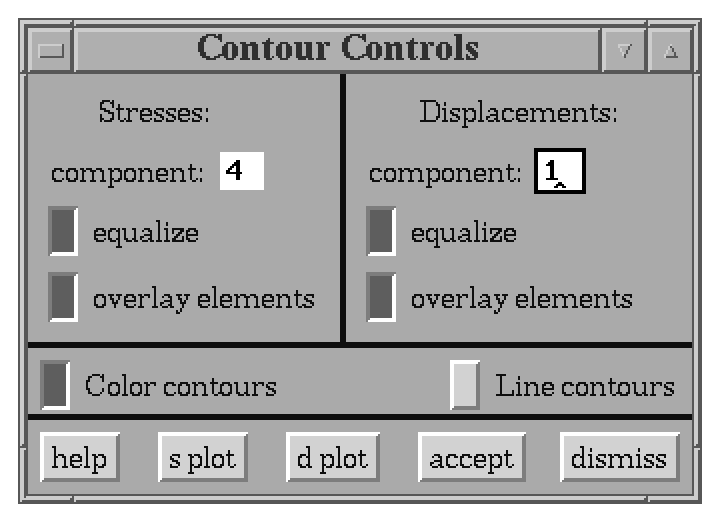
\includegraphics[width=2.82in]{figures/velvet_contour}
\end{center}
\caption{The control dialog box for contour plots.}
\label{velvet.contour}
\end{figure}

Other contouring controls include toggles for histogram equalization and
element boundary overlay.  Histogram equalization is a standard technique
in image processing for enhancing the contrast of images.  If the overlay
elements toggle is checked then the outline of all the elements in the problem
will be drawn in black on top of the color image.  An example of stress
contours (rendered here in greyscale) for the wrench example pictured
earlier is shown in Figure~\ref{velvet.stresses}.  Note that both histogram
equalization and element overlay were enabled for this plot.

In addition to the standard buttons for {\bf help}, {\bf accept}, and
{\bf dismiss}, you can use the {\bf s plot} and {\bf d plot} buttons as
an alias for selecting either {\bf plot stresses} or {\bf plot displacements}
from the main {\bf postprocessing} menu item.  Both buttons cause the
dialog state to be accepted before the plot is generated.

\begin{figure}
\begin{center}
 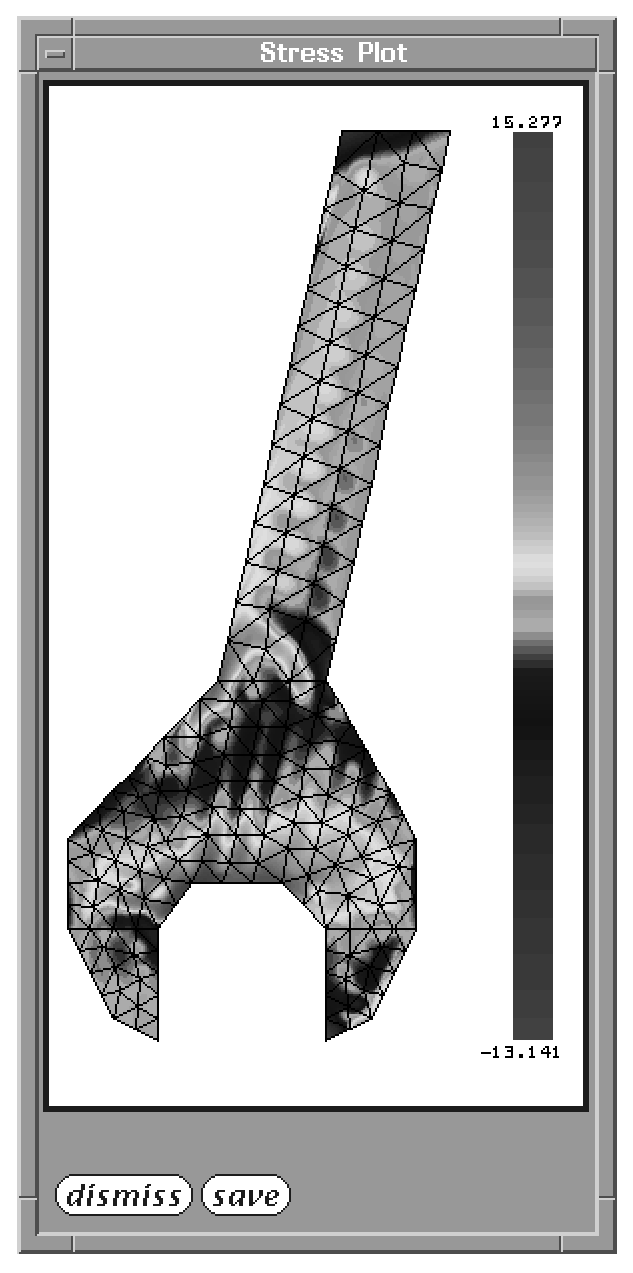
\includegraphics[width=6in]{figures/velvet_stresses}
\end{center}
\caption{The stress output window for the wrench example.}
\label{velvet.stresses}
\end{figure}

\subsection{Controlling structure plots}

Additional control over structure plots is available through the wireframe
dialog box (Figure~\ref{velvet.wireframe}).  The majority of these controls 
are specific to three-dimensional visualization.  The three dial widgets 
control the rotation of the drawing about the three spatial axes.  The 
magnification determines the multiplicative factor by which nodal 
displacements will be increased before the nodes are plotted.  z scaling 
controls the front to back aspect ratio of the resulting plot.  The toggle
for hidden line removal is non-functional in the current version of
{\em velvet}.  The defaults reflected in the dialog pictured in 
Figure~\ref{velvet.wireframe} were used to generate our earlier example 
of the structural plot of the bicycle (Figure~\ref{velvet.structure}). 

The extra button at the bottom of the dialog {\bf plot} is equivalent to
pressing {\bf accept} and selecting {\bf plot structure} from the 
{\bf postprocessing} menu.

\begin{figure}
\begin{center}
 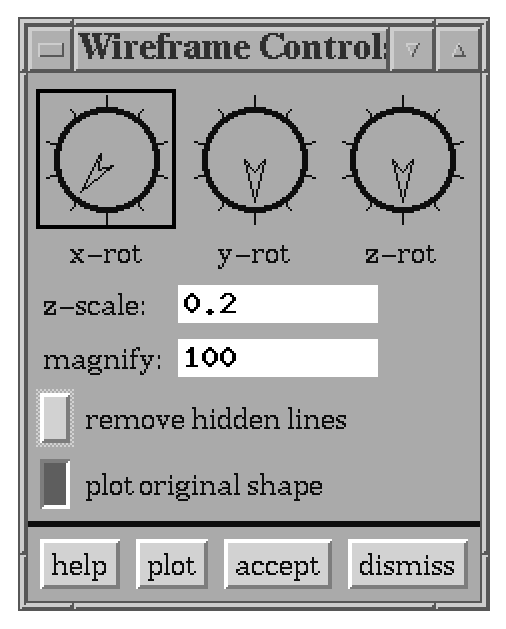
\includegraphics[width=1.86in]{figures/velvet_wireframe}
\end{center}
\caption{The wireframe plotting control dialog box.}
\label{velvet.wireframe}
\end{figure}

\subsection{Controlling animation}
The analysis parameters used in constructing a displacement table for
an animation are the same as those that would be used in a normal solution
for that problem in transient analysis mode, except for the nodes and DOF.
As mentioned above, an animation will automatically solve for all nodes
at the x and y (and z if the problem is 3d) translational DOF.  The 
magnification of the displacements during the animation can be controlled 
via the same magnification control that is used in structure plots.  Likewise 
for 3-d animations, the 3-d drawing parameters will be taken from the 
controls in the wireframe control dialog box.
